\section{Anwendung ausserhalb der Medizin \label{chapter:MRI:bsp}}

Im folgenden Abschnitt wird die Anwendung des Prinzips ausserhalb der Medizin erl"autert. Er unterteilt sich in die beiden Unterkapitel "`Wasserstoff als Signalgenerator"' und "`NMR-Spektrum"'. Die theoretischen Grundlagen zu diesem Kapitel wurden im Kapitel\;\ref{sec:quant} erl"autert.

\subsection{Wasserstoff als Signalgenerator}
Die Motivation war herauszufinden, ob es m"oglich ist, Fossilien in einem Stein zu erkennen. Die Problematik in diesem Fall ist, dass es sich um Materialien handelt, die arm an Wasserstoffatomen sind, welche f"ur die Bildgebung eine massgebende Rolle spielen. Wie in Tabelle\;\ref{mri:bsp:tab:NMR_Kerne} ersichtlich, ist das abgegebene Signal der Nicht-Wasserstoffatome massiv geringer. Aus diesem Grund werden nur H-Atome benutzt, um MRI Bilder zu generieren. Daraus folgt, dass das MRI nicht geeignet ist zur Erzeugung von Bildern im Stein verborgener Knochen. Es ist zwar heutzutage m"oglich 3D-Bilder vom Inneren eines Steines zu machen, jedoch nutzen alle Ger"ate R"ontgenstrahlen, welche ohne Hilfe des Kernspins auskommen.
\begin{table}[h]
	\centering
	\begin{tabular}{|c|c|c|c|}
		\hline
		Kern 				& $\omega_0$ 	& Relative 				& Relatives\\
							& @ 1.5T [MHz] 	& Signal-Intensit"at 	& Gesamt Signal\\
		\hline
		$\mathrm{^{1}H}$ 	& 63.8 			& 1.000 				& 1.000 \\
		$\mathrm{^{13}C}$ 	& 16.1 			& 0.016 				& 0.0000001 \\
		$\mathrm{^{19}F}$ 	& 60.1 			& 0.833 				& 0.000001 \\
		$\mathrm{^{31}P}$ 	& 25.8 			& 0.066 				& 0.00001 \\
		\hline
	\end{tabular}
	\caption{Relative Empfindlichkeit einiger NMR-Kerne \cite{skript:mri:AMSM_Paper}}
	\label{mri:bsp:tab:NMR_Kerne}
\end{table}
Doch weshalb ist das Signal der Wasserstoffatome so viel klarer und st"arker als die Signale der anderen Atome? Bei genauerer Betrachtung der Tabelle\;\ref{mri:bsp:tab:NMR_Kerne} l"asst sich feststellen, dass die relative Signal-Intensit"at des "`Fluor 19"' Atoms der des Wasserstoff Atoms am n"achsten kommt. Wenn man davon ausgehen darf, dass Kerne "ahnlich wie Atome eine Schalenstruktur aufweisen, dann hat Fluor-19 wahrscheinlich eine ziemlich spezielle Struktur, weil sich mit 18 Nukleonen eine stabile Konfiguration erzielen l"asst -- ebenso wie mit 18 Elektronen (bei Argon). Das 19. Nukleon ist daher in einer neuen Schale relativ exponiert, und d"urfte sich "ahnlich wie das nackte Proton eines Wasserstoffkerns verhalten. Da Fluor im Vergleich zum Wasserstoff relativ selten auf der Erdkruste und erst recht in Menschen oder Tieren vorhanden ist, stellen sich die H-Atome als perfekte Signalgeneratoren dar und "uberbieten die F-Atome. 

\subsection{NMR-Spektrum}
Obwohl das Prinzip des MRI ausserhalb der Medizin keinen grossen Anklang fand, wird in einigen Labors diese Methode zur Analyse von Stoffen genutzt. Die meist von Chemikern eingesetzte Maschine -- der eigentliche Vorg"anger des MRIs -- ist unter dem Namen NMR-Spektrometer bekannt. Dieser arbeitet mit Feldern von bis zu 21 Tesla, was im Vergleich zur Medizin, die typischerweise MRI-Ger"ate einsetzt, welche Felder zwischen 0.5 und 3 Tesla\footnote{Ein paar wenige Kliniken besitzen MRI-Ger"ate mit 7 - 9 Tesla} generieren, um einiges st"arker ist. Das Feld bei einer Kernspinresonanzspektroskopie, kurz NMR-Spektroskopie (von der englischen Bezeichnung ”nuclear magnetic resonance“), wird meistens in einem Loch von der Gr"osse eines Reagenzglases erzeugt. Ein Beispiel eines solchen Ger"ats ist auf der Abbildung\;\ref{mri:bsp:abb:nmr_Beispiel} zu sehen. 
\begin{figure}[h]
	\centering
	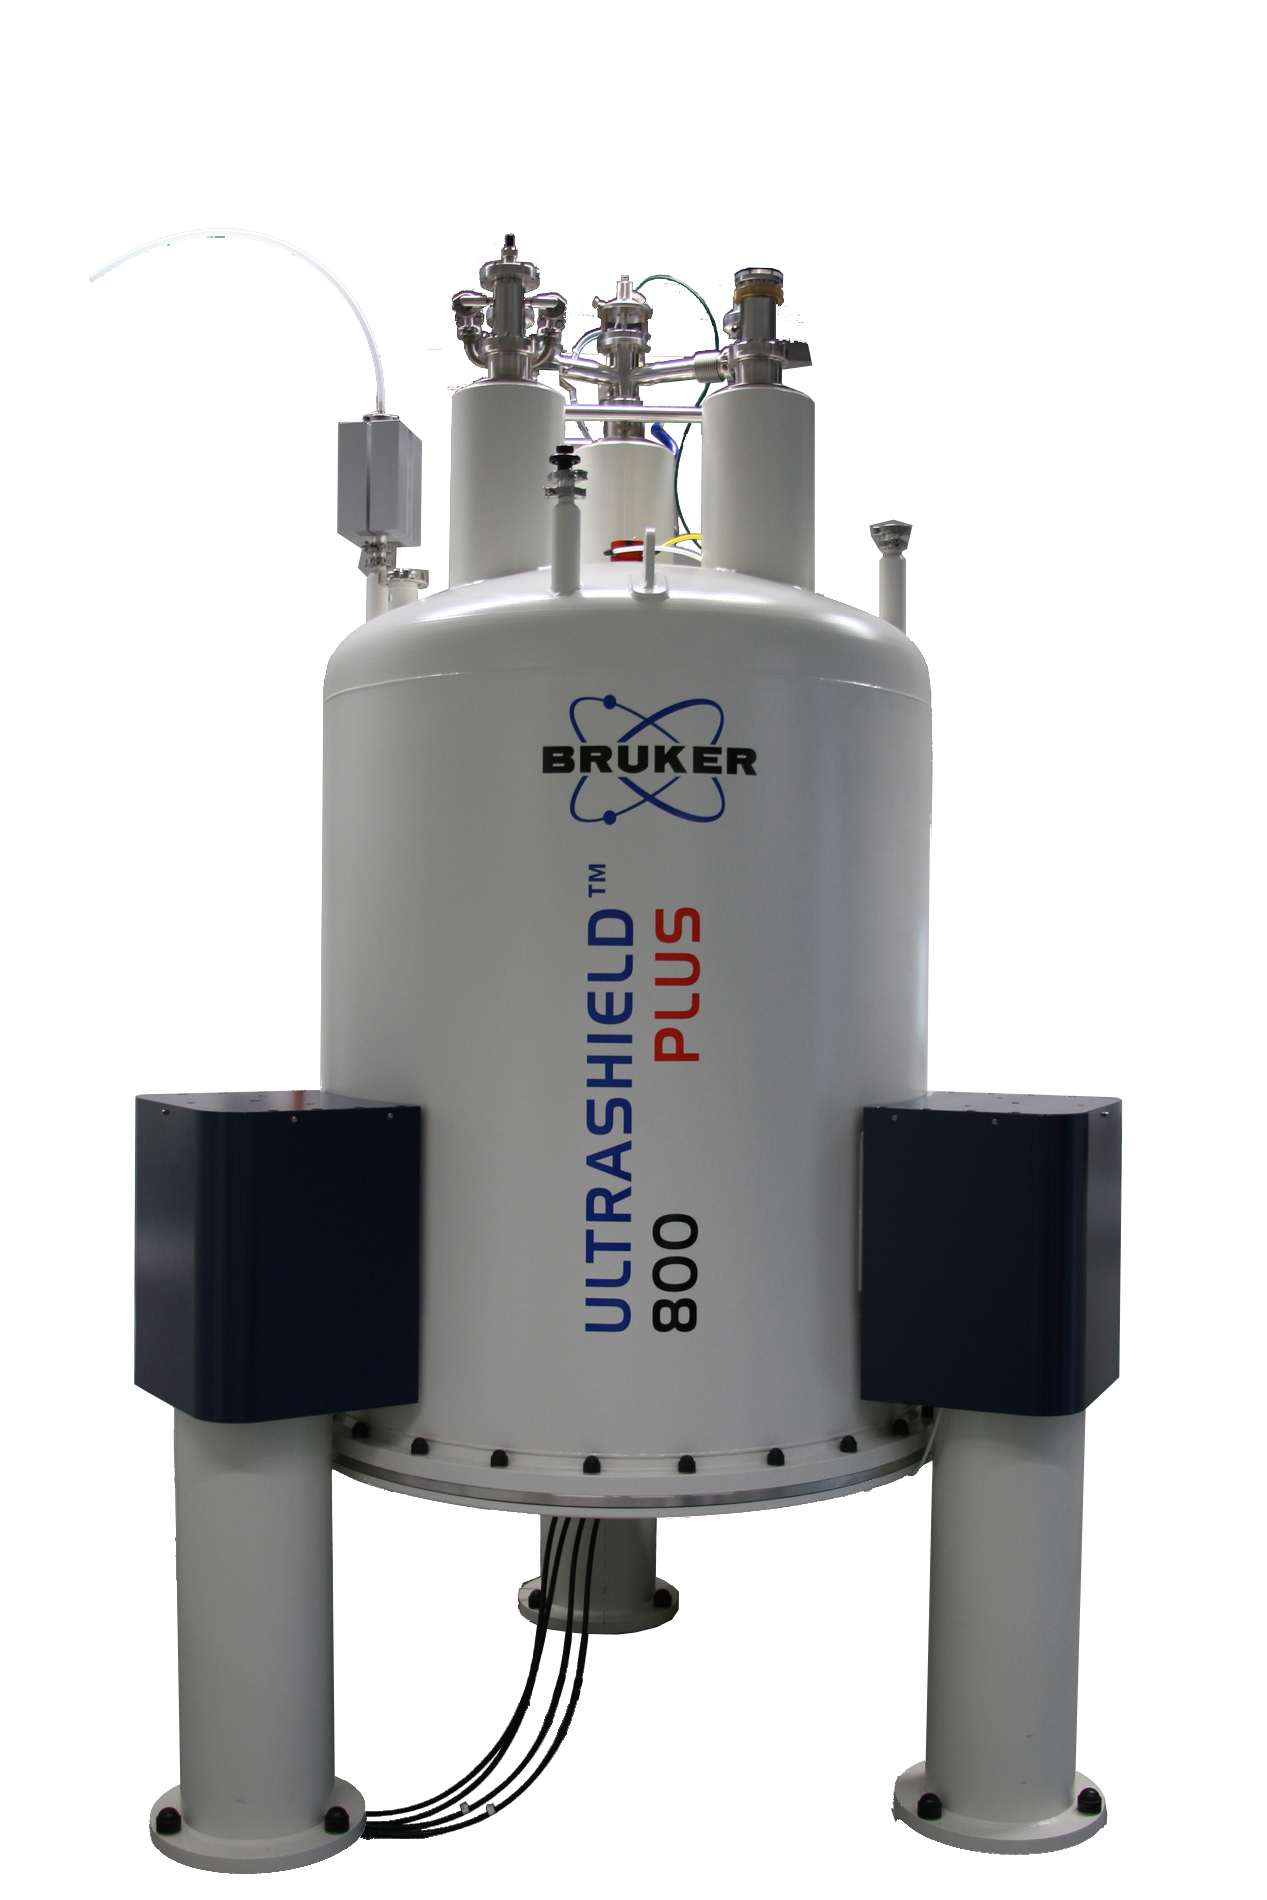
\includegraphics[width = 3cm]{./mri/pic/NMR.png}
	\caption{Beispiel eines NMR-Ger"ates \cite{skript:mri:MaxPlanckCampus}}
	\label{mri:bsp:abb:nmr_Beispiel}
\end{figure}

\subsubsection{Bildausgabe}
Das Bild, welches bei einem NMR-Spektrometer entsteht, sieht nicht etwa so aus wie das eines MRI (siehe Abbildung \ref{mri:abb:kiwi} / \ref{mri:abb:ananas}), sondern gibt ein Spektrum wieder. Die Abbildung\;\ref{mri:bsp:abb:Etanolspektrum} zeigt eines der ersten NMR-Spektren, f"ur welches Edward Mills Purcell zusammen mit Felix Bloch 1952 den Nobelpreis f"ur Physik bekamen. Im aktuellen NMR-Spektren ist die Abszisse gespiegelt, d.h. sie geht von tieferen zu h"oheren Frequenzen. Was auf dieser Spektrum direkt zu sehen ist, sind die drei verschieden hohen Signale, welches vom NMR aufgenommen wurden. Das h"ochste Signal geh"ort dem $\mathrm{CH_3}$-Teil des Molek"uls, da dieser Molek"ul-Abschnitt die meisten H-Atome besitzt und somit das h"ochste magnetische Potenzial. Analog dazu lassen sich die zwei weiteren Ausschl"age des $\mathrm{CH_2}$- und OH-Teiles zu interpretieren. 
\begin{figure}[h]
	\centering
	\begin{minipage}{0.55\textwidth}
		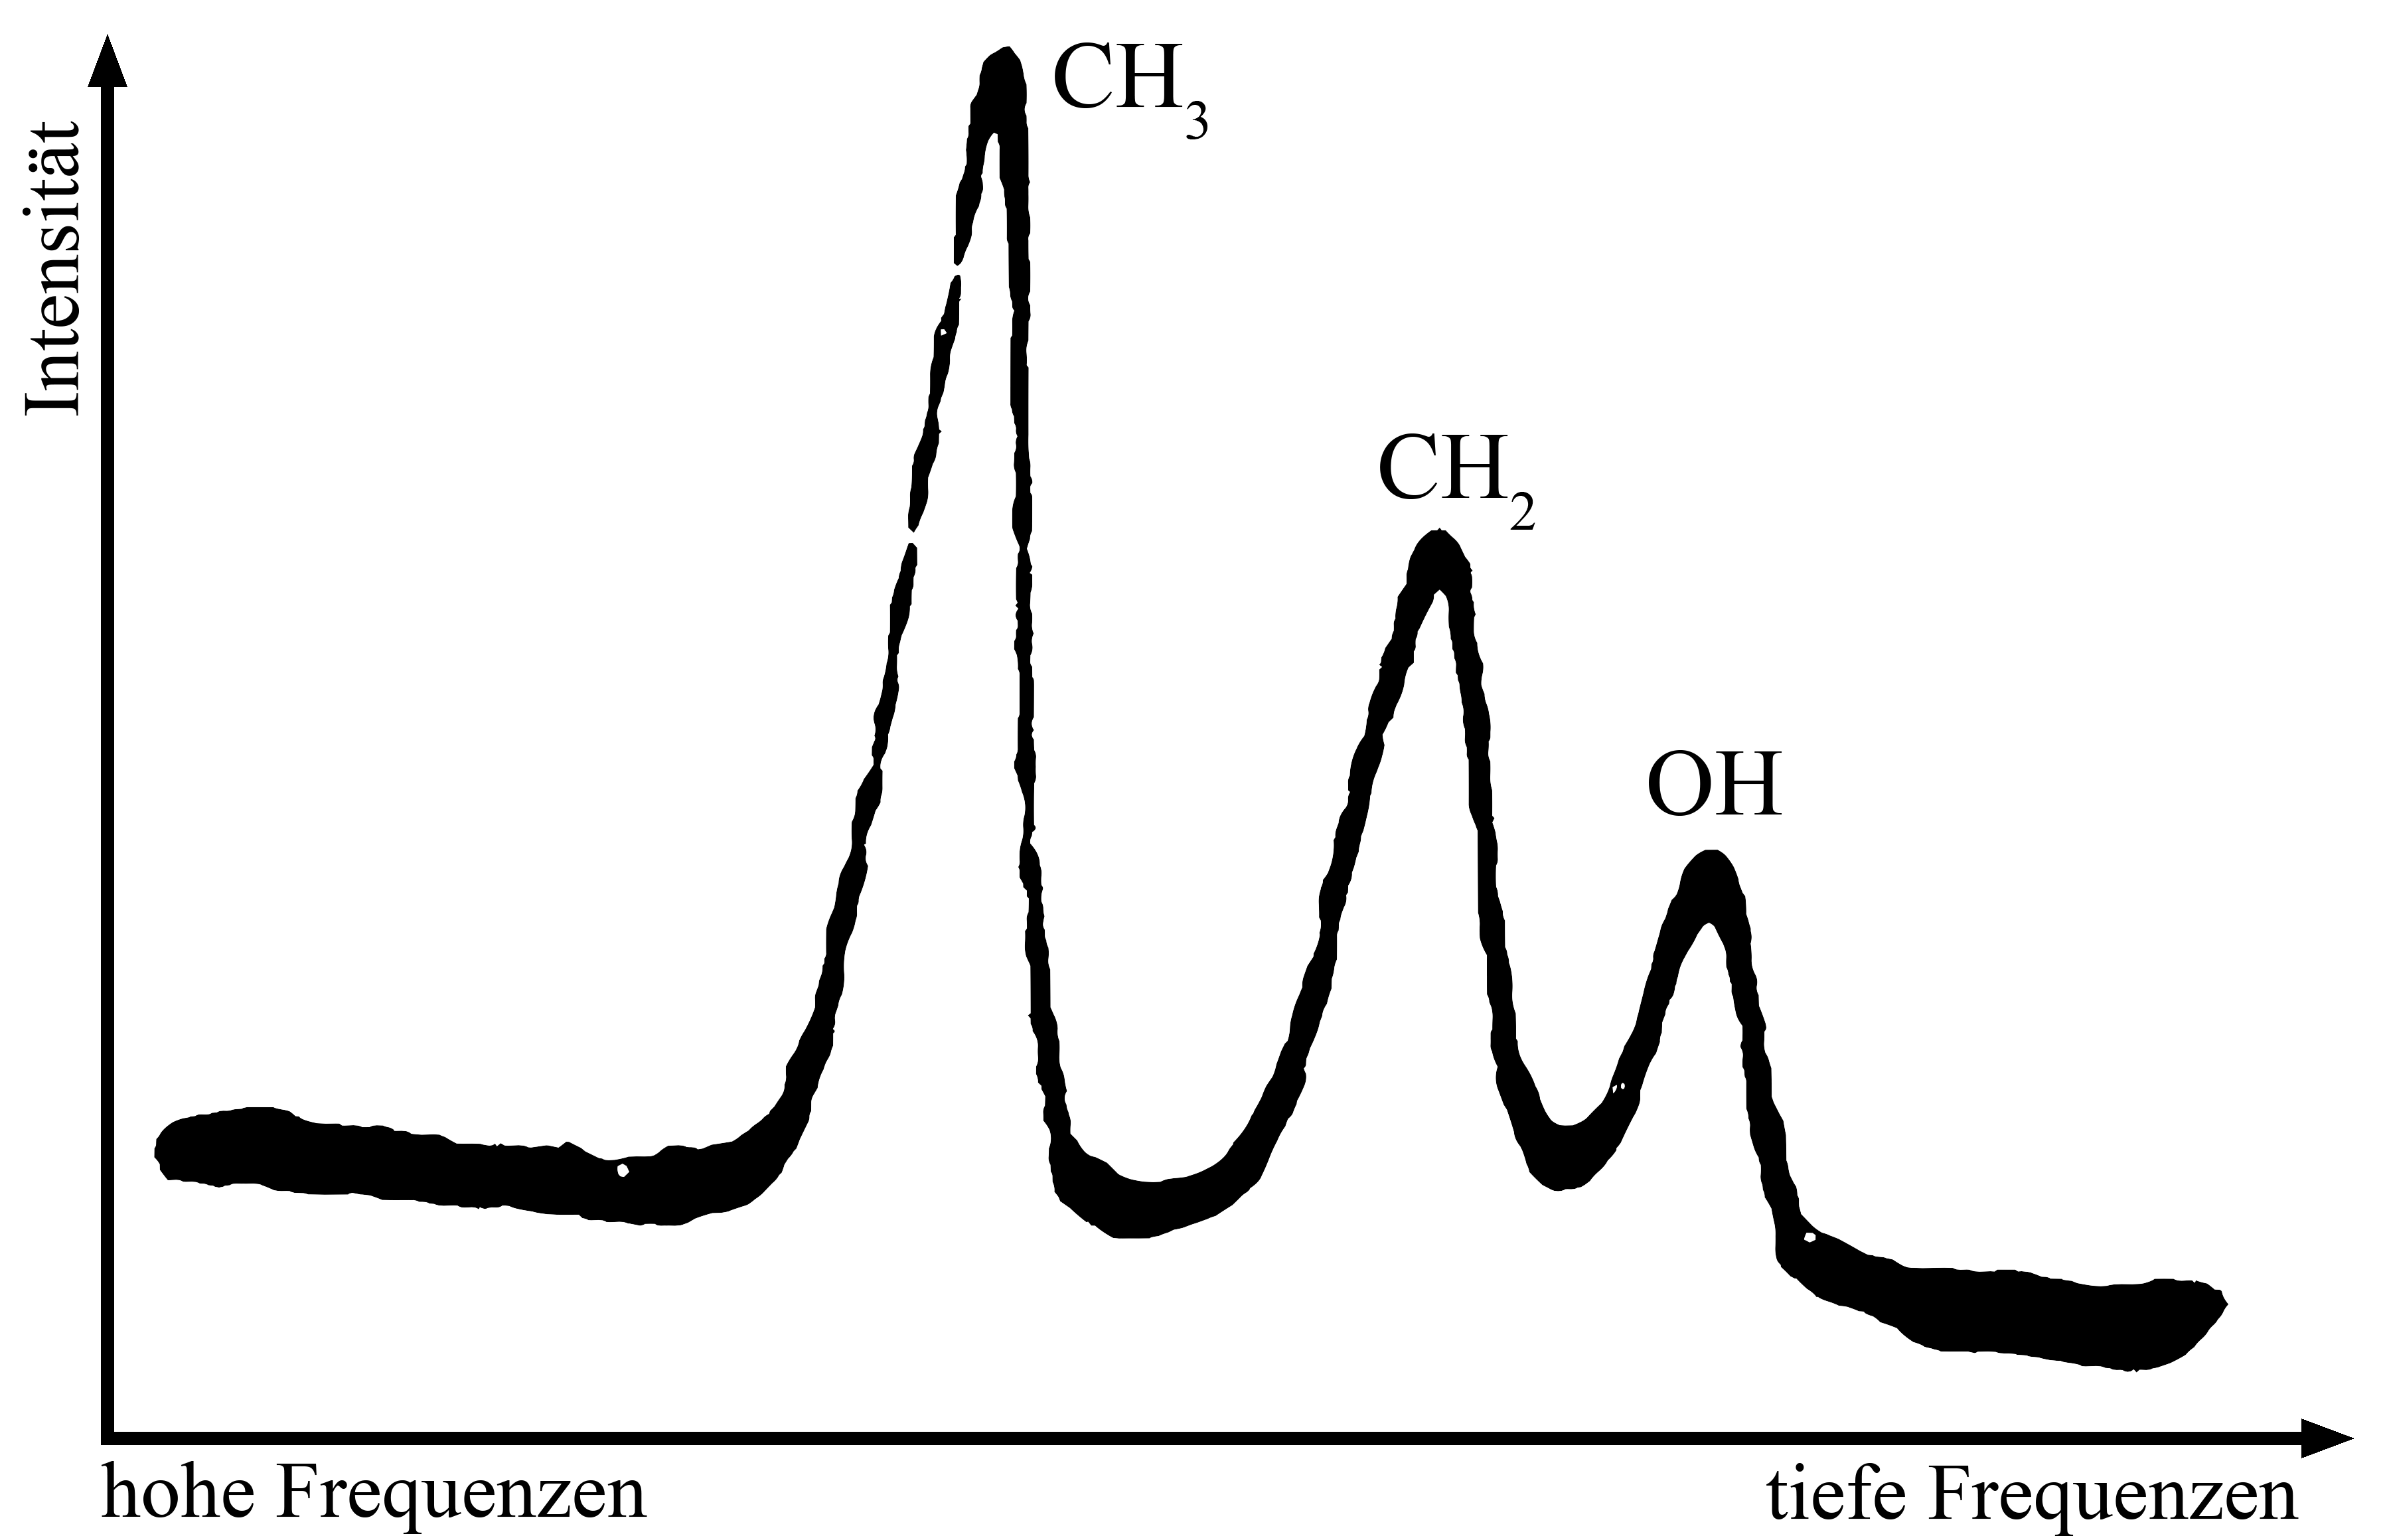
\includegraphics[width = \textwidth]{./mri/pic/CW_SpektrumEthanol.png}
	\end{minipage}
	\begin{minipage}{0.42\textwidth}
		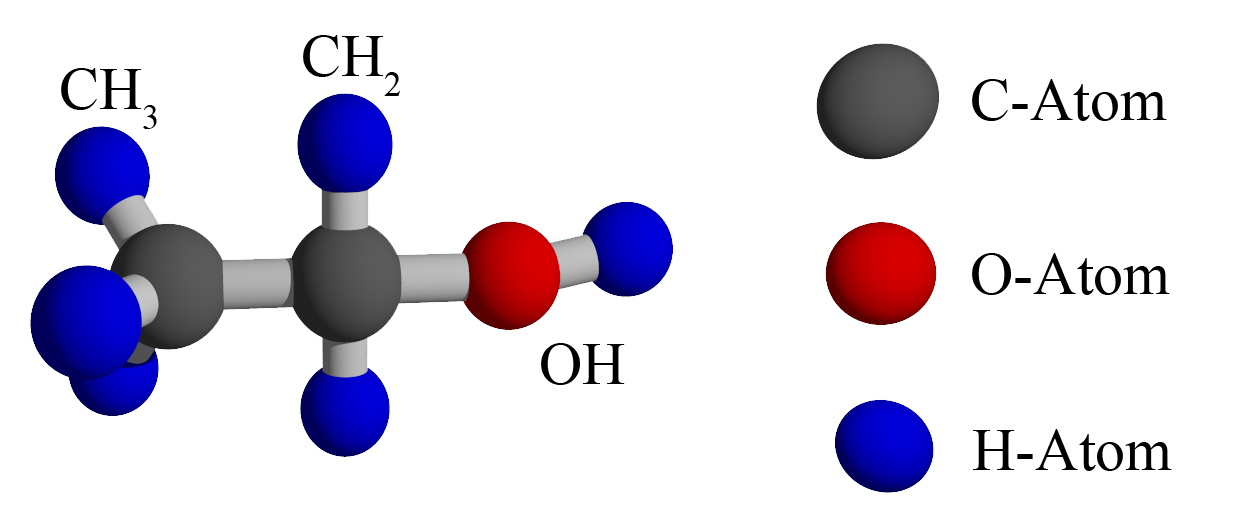
\includegraphics[width = \textwidth]{./mri/pic/Ethanol.png}
	\end{minipage}
	\caption{Ethanol NMR-Spektrum \cite{skript:mri:NMRSkopie} und ein Ethanolmolek"ul}
	\label{mri:bsp:abb:Etanolspektrum}
\end{figure}
Die Verschiebung der Frequenz (Abweichung auf der $x$-Achse) ist schwieriger zu verstehen, da es sich hier um Wasserstoffatome handelt, die das Signal abgeben. Diese geben wiederum -- wie in Tabelle\;\ref{mri:bsp:tab:NMR_Kerne} ersichtlich -- immer bei der gleichen Frequenz Signale ab. In der Chemie, wo auch die meisten NMR-Ger"ate eingesetzt werden, wird f"ur dieses Ph"anomen das Sauerstoff-Atom verantwortlich gemacht. Bei diesem Atom handelt es sich um ein elektronengieriges, d.h. dass dieses die Elektronen des direkt angeschlossenen Wasserstoffatomes stark anzieht und somit eine Art Abschirmung gegen aussen erzeugt, was wiederum die Frequenz beeinflusst. Die zwei Wasserstoff-Atome des $\mathrm{CH_2}$-Teils hingegen sind "uber das Kohlenstoff-Atom etwas abgekoppelt. Nichts desto trotz k"onnen sie den Einfluss des O-Atoms immer noch sp"uren, w"ahrend die H-Atome des $\mathrm{CH_3}$-Teiles fast nichts mehr vom Sauerstoff-Atom mitbekommen. Die Chemiker nennen es eine Elektronen Wolke, die um das O-Atom entsteht, welche wiederum wie ein Schild wirkt.

\subsubsection{Heutiger Einsatz in der Chemie}
Die Abbildung \ref{mri:bsp:abb:EtanolspektrumNew} zeigt ein aktuelles Spektrum des Ethanols. Dieses genauer zu erkl"aren w"urde jedoch den Rahmen dieses Artikels sprengen, denn hier sind bereits die Kopplungen der H-Atomen zu den benachbarten Segmenten herauslesen. Was aber deutlich zu erkennen ist, ist die feinere Aufl"osung. Dank des Fortschritts, welcher bis jetzt gemacht werden konnte, erlauben diese NMR-Spektren den Chemikern Stoffe bis in die molekulare Ebene zu untersuchen und zu bestimmen. 
\begin{figure}[h]
	\centering
	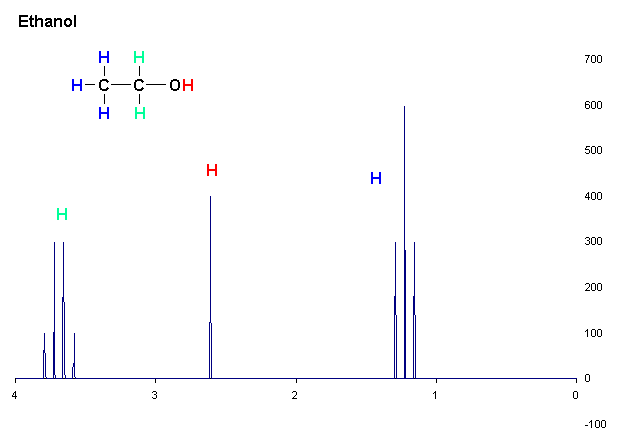
\includegraphics[width = 0.75\textwidth]{./mri/pic/CW_SpektrumEthanol_Neu.png}
	\caption{Aktuelles Ethanol NMR-Spektrum \cite{skript:mri:EthanolNeu}}
	\label{mri:bsp:abb:EtanolspektrumNew}
\end{figure}